Serverless computing has become a key model for developing and deploying cloud applications, offering a zero-administration approach by fully decoupling backend infrastructure management from application development. In this model, applications are composed of small, stateless functions or handlers that operate independently and execute in response to specific events. Cloud providers run these handlers in isolated sandboxes, such as \textbf{containers}, allowing for both \textbf{secure isolation} and \textbf{efficient autoscaling}, while enabling a genuine pay-as-you-go billing model.\vspace{14pt}\\
The architecture of a serverless platform is illustrated in Fig. 1. In this setup, the serverless platform receives an event sent via HTTP or another cloud-based source. Internally, the platform includes an event queue, a dispatcher, and worker nodes. Upon receiving a request, the system identifies the appropriate function(s) to handle the event. The dispatcher then routes the request to a worker node, retrieving the necessary function code from a database.\vspace{14pt}\\
The worker node executes the function(s), launching one or more instances depending on the request volume and available resources. If resources are sufficient, function instances (typically run in containers) are launched with restricted resources to carry out the task. If resources are limited, the function request is queued until resources become available.\vspace{10pt}\\
\begin{center}
    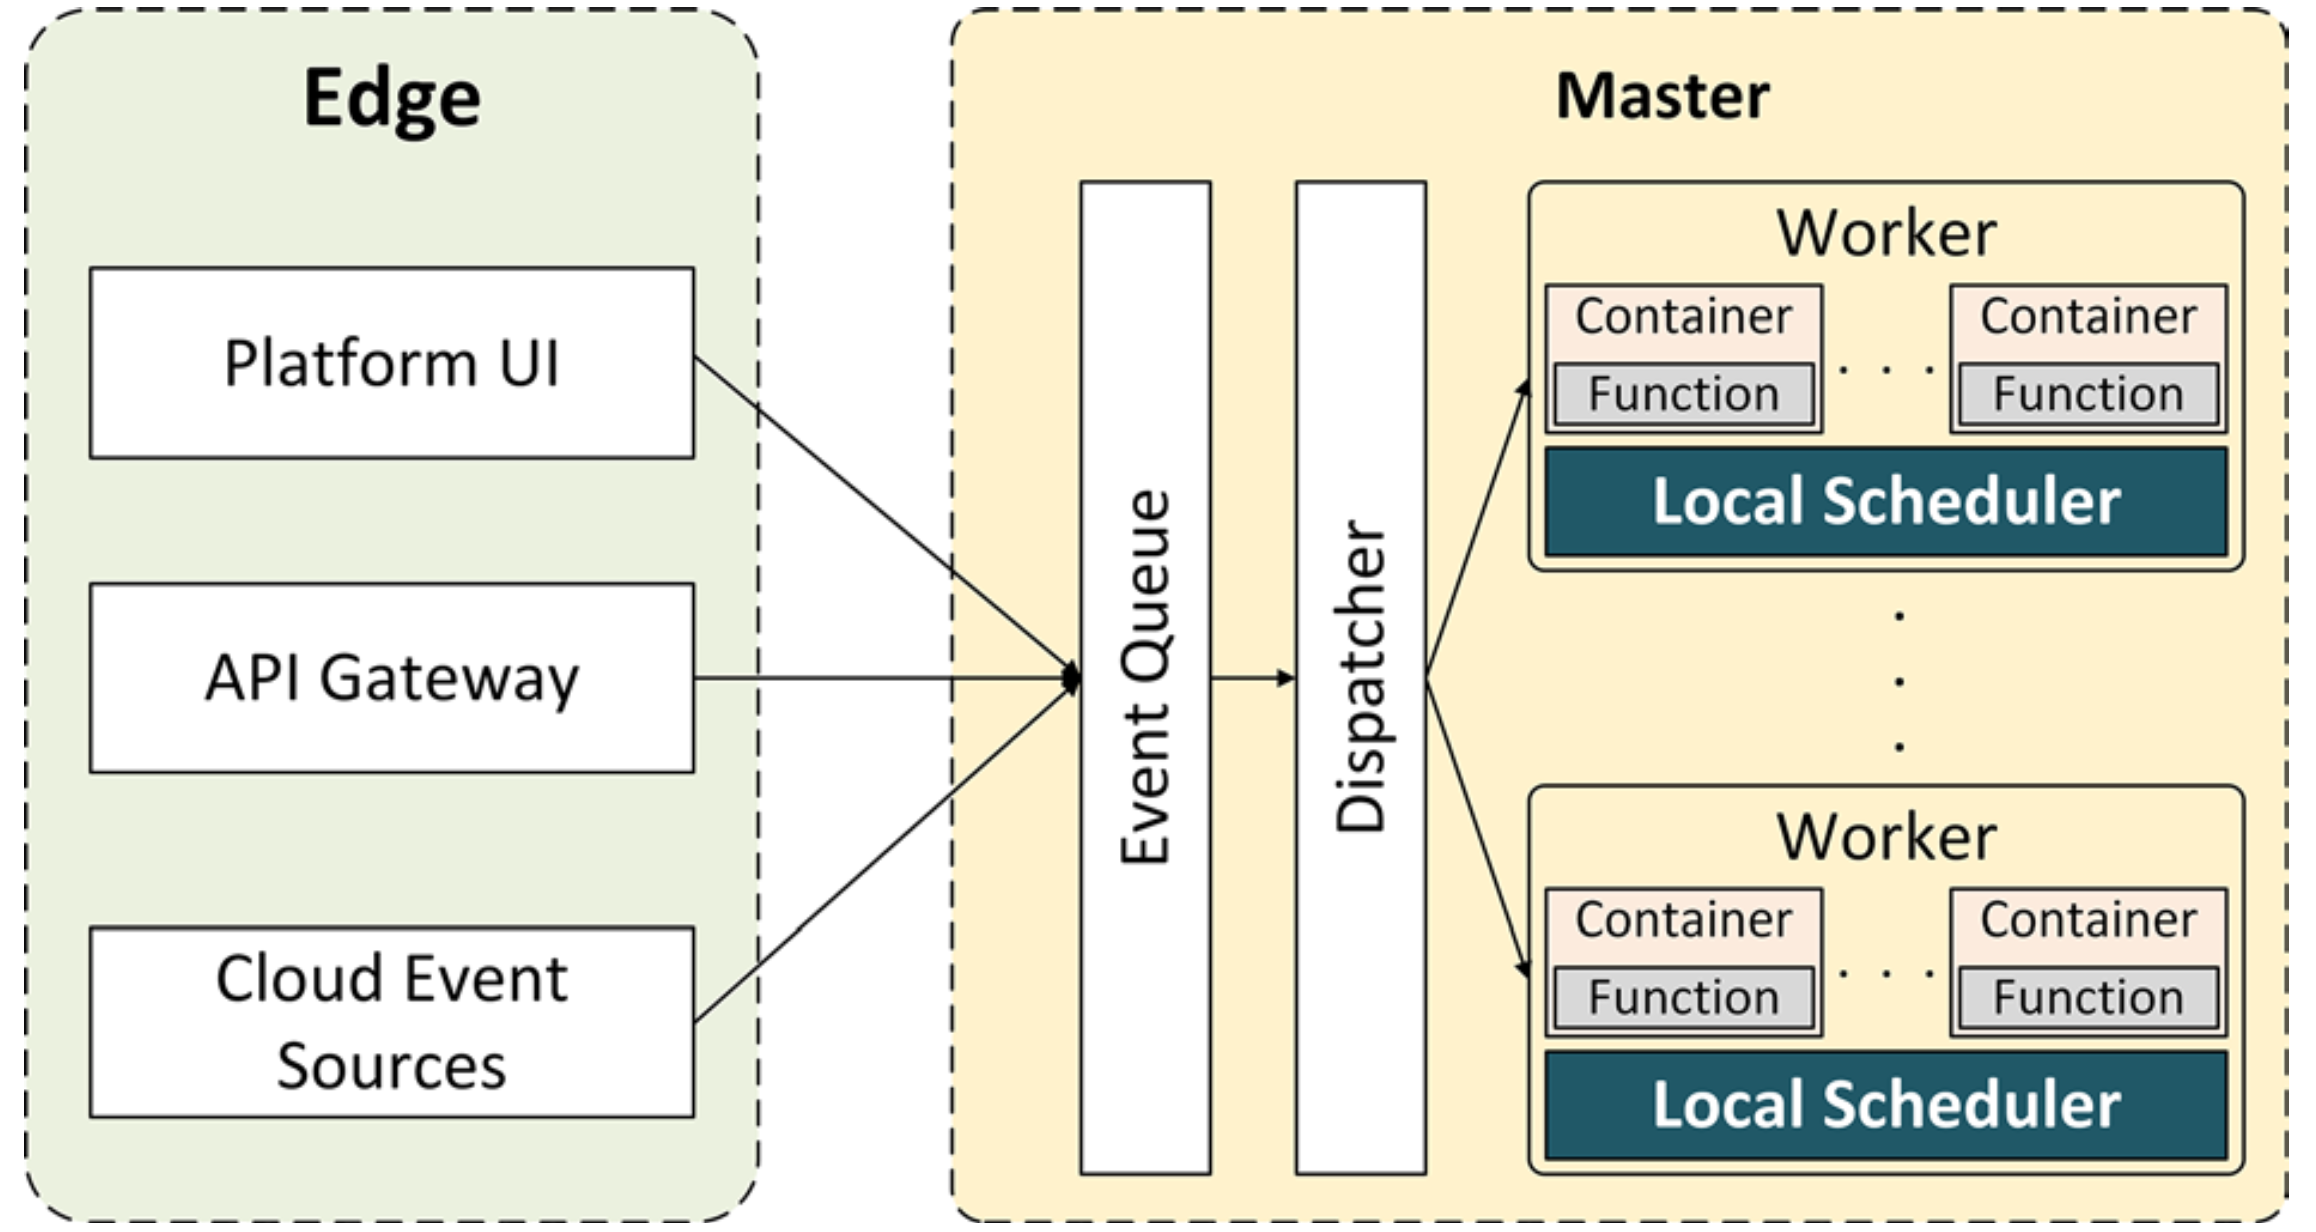
\includegraphics[width=0.7\textwidth]{img/arch.png}
    \captionof{figure}{Blueprint of serverless platform architecture}
    \vspace{10pt}
\end{center}
A smart load balancer helps prevent workers from becoming overloaded. However, under high invocation rates or sudden bursts, a long execution queue can lead to significant wait times. Additionally, when resources are optimized to use the fewest nodes, some functions may experience delays, affecting \textbf{Quality of Service} (\textbf{QoS}). Consequently, the local scheduling approach plays a critical role in optimizing average function wait times, throughput, and resource utilization at worker nodes.\vspace{14pt}\\
Starting a new instance requires initializing the container with necessary libraries, which can introduce startup latency -- commonly known as a \textbf{cold start}. To reduce cold start delays, cloud providers often keep instances paused after use so they can be quickly reused for future invocations. After a function completes or reaches its maximum execution time, the worker node collects execution logs and makes the results available to the user. Scale-to-zero functionality allows users to pay only for the exact time and resources used during active function execution.\cite{banaei2022etas}